\section{Material moved from the main text of the shortened version}
\label{sec:s-moved}
The shortened manuscript (\texttt{main\_access\_v2.tex}) moved the following secondary tables and details here. Their content and numbers are unchanged from the full-length version.

\subsection{Main terms and notation}
\begin{table}[h]
\centering
\caption{Main terms and notation.}
\footnotesize
\begin{tabular}{@{}p{0.27\textwidth}p{0.66\textwidth}@{}}
\toprule
Term & Meaning \\
\midrule
Session (episode) & One recorded play-through of one game, logged about once per second; one episode of the decision process. \\
Linkage group & Sessions that may come from the same person; the unit of every split. \\
Event second, $y_t$ & $y_t=1$ if the discomfort reported at second $t$ is at least 1 (slight), otherwise $y_t=0$. \\
State $s_t$ & Causal feature vector at second $t$, computed from seconds $0,\dots,t$ of the same session only. \\
Action $a_t$ & $1$ = raise an alarm, $0$ = stay silent. \\
Reward $R(a,y)$ & $R(1,1)=+0.5$, $R(0,0)=+0.1$, $R(0,1)=-0.5$, $R(1,0)=-0.1$. \\
Regrets $\Delta_{\mathrm{FN}}$, $\Delta_{\mathrm{FP}}$ & Reward lost by a missed event (1.0) and by a false alarm (0.2). \\
$Q(s,a)$, $\Delta Q(s)$ & Action value; decision margin $Q(s,1)-Q(s,0)$. \\
Score $\hat p(s)$ & A model's output mapped to the nominal scale of $P(y=1\mid s)$. \\
5:1 cost $c$ & $(5\,\mathrm{FN}+\mathrm{FP})/N$. \\
OOF prediction & Out-of-fold prediction: the score of an inner-validation second from a model not trained on its group. \\
Operating rule & How the alarm threshold on $\hat p$ is chosen: D1 (minimum validation 5:1 cost; primary), D0 ($\hat p\ge1/6$) or a validation recall constraint. \\
\bottomrule
\end{tabular}
\end{table}

\subsection{Research gaps}
\begin{table}[h]
\centering
\caption{Gaps in the evaluation of asymmetric-reward cybersickness detectors and how this study addresses them (references as in the main text).}
\footnotesize
\begin{tabular}{p{0.22\textwidth}p{0.26\textwidth}p{0.44\textwidth}}
\toprule
Gap & Evidence & This study \\
\midrule
Splits of 1-Hz session data without session separation & 70/30 split without reported session separation on the same gameplay data (TruVR, Kundu et al.); leakage literature (Kapoor and Narayanan; Kaufman et al.; Roberts et al.) & Session-linkage groups, nested grouped evaluation, train-only preprocessing, protocol fixed before testing; effect of the split protocol reported \\
Relation of asymmetric rewards to cost-sensitive learning left implicit & DQN classifiers for imbalanced data (Lin et al.; Yang et al.) & Derivation from known results that the 5:1 reward equals the 5:1 cost-sensitive Bayes threshold, and of how error-triggered termination departs from it \\
RL detectors not compared with matched cost-sensitive or minimal baselines & -- & Seven models with the same search procedure, number of configurations and decision rules; two exposure-time baselines; group-bootstrap and exact sign-flip inference with multiplicity adjustment \\
Robustness assessed with optimization-based input attacks only & Kundu et al.; Ahmed et al. & Bounded, physically motivated telemetry perturbations as a sanity check, with adaptive evasion and false-alarm worst cases \\
\bottomrule
\end{tabular}
\end{table}

\subsection{Expected cost under three operating rules}
\begin{table}[h]
\centering
\caption{Expected 5:1 cost (mean over seeds) under three operating rules chosen without test data.}
\footnotesize
\begin{tabular}{lccc}
\toprule
Model & D1: min cost & D0: $\hat p\ge 1/6$ & val.\ recall $\ge$ 0.95 \\
\midrule
E-DDQN & \EDDQNCostCostMean & \EDDQNBayesCostMean & \EDDQNRecCostMean \\
E-CB & \ECBCostCostMean & \ECBBayesCostMean & \ECBRecCostMean \\
DQN & \DQNCostCostMean & \DQNBayesCostMean & \DQNRecCostMean \\
CS-MLP & \CSMLPCostCostMean & \CSMLPBayesCostMean & \CSMLPRecCostMean \\
LogReg & \LRCostCostMean & \LRBayesCostMean & \LRRecCostMean \\
HGB & \HGBCostCostMean & \HGBBayesCostMean & \HGBRecCostMean \\
RF & \RFCostCostMean & \RFBayesCostMean & \RFRecCostMean \\
\midrule
Always alarm & \AlwaysCost & \AlwaysCost & \AlwaysCost \\
\bottomrule
\end{tabular}
\end{table}

\subsection{Matched operating points}
Thresholds were chosen on validation predictions to reach the stated recall or specificity (descriptive, no test). The thresholds transfer worst for E-DDQN: at both recall targets shown, and also at 0.80 and 0.99 (released results), it attains lower test recall than every supervised model, and at the 0.95 target also a higher false-positive rate. Read from the ROC curves at fixed recall (descriptive), the false-positive rate at 95\,\% recall is \EDDQNRocFPRatNineFive\,\% for E-DDQN and \RFRocFPRatNineFive\,\% for the random forest.
\begin{table}[h]
\centering
\caption{Matched operating points: test recall (\%), false-positive rate (\%) and false-positive count of the seed ensemble at validation-chosen thresholds.}
\footnotesize
\begin{tabular}{lccccccccc}
\toprule
 & \multicolumn{3}{c}{val. recall $\ge$ 0.90} & \multicolumn{3}{c}{val. recall $\ge$ 0.95} & \multicolumn{3}{c}{val. specificity $\ge$ 0.80} \\
Model & Rec. & FPR & FP & Rec. & FPR & FP & Rec. & FPR & FP \\
\midrule
E-DDQN & 81.7 & 77.0 & 4,036 & 84.5 & 86.6 & 4,539 & 25.2 & 18.6 & 974 \\
E-CB & 88.6 & 68.0 & 3,565 & 92.4 & 78.1 & 4,093 & 31.2 & 17.4 & 910 \\
DQN & 88.0 & 64.2 & 3,366 & 91.7 & 72.7 & 3,810 & 32.2 & 14.2 & 743 \\
CS-MLP & 94.1 & 78.4 & 4,111 & 97.5 & 85.1 & 4,463 & 24.2 & 12.7 & 666 \\
LogReg & 92.8 & 73.5 & 3,856 & 97.2 & 81.7 & 4,285 & 37.7 & 22.5 & 1,181 \\
HGB & 95.4 & 72.2 & 3,785 & 97.5 & 81.7 & 4,282 & 24.3 & 11.3 & 594 \\
RF & 93.7 & 64.0 & 3,358 & 96.9 & 74.3 & 3,896 & 21.0 & 13.3 & 695 \\
\bottomrule
\end{tabular}

\end{table}

\subsection{Selection optimism}
\begin{table}[h]
\centering
\caption{Pooled inner-validation 5:1 cost of the selected configuration (search seed, at its cost-minimizing threshold) versus its outer-test cost (seed ensemble, rule D1), averaged over the five outer folds (unweighted fold means, which differ from the pooled costs of the main results table).}
\footnotesize
\begin{tabular}{lccc}
\toprule
Model & Inner-OOF cost at selection & Outer-test cost & Gap \\
\midrule
E-DDQN & 0.467 & 0.754 & +0.288 \\
E-CB & 0.488 & 0.557 & +0.070 \\
DQN & 0.478 & 0.544 & +0.065 \\
CS-MLP & 0.501 & 0.534 & +0.033 \\
LogReg & 0.518 & 0.531 & +0.014 \\
HGB & 0.518 & 0.539 & +0.021 \\
RF & 0.495 & 0.481 & $-$0.015 \\
\bottomrule
\end{tabular}

\end{table}

\subsection{Reward-ratio sensitivity}
The regret ratio of E-DDQN's reward was varied from 1:1 to 10:1 with the selected configuration per fold fixed (ratio 5:1 reproduces the main E-DDQN run bit for bit). The nominal greedy cut-off is $1/(1+R)$; under class-balanced replay it corresponds approximately to $1/(1+kR)$ on $P(y=1\mid s)$, with $k=$ \SSEDDQNKMin--\SSEDDQNKMax. Recall of the greedy policy rises from \RatioArgOneRecall\,\% (1:1) to \RatioArgFiveRecall\,\% (5:1) and \RatioArgOneZeroRecall\,\% (10:1), while specificity falls from \RatioArgOneSpec\,\% to \RatioArgFiveSpec\,\% and \RatioArgOneZeroSpec\,\%. With validation-chosen thresholds all ratios end at similar costs (\RatioTunedOneCost--\RatioTunedOneZeroCost; the largest difference is smaller than any ratio's seed SD; no formal test).
\begin{table}[h]
\centering
\caption{Reward-ratio sensitivity of E-DDQN: greedy (arg-max) policy and validation-tuned threshold (rule D1); mean ($\pm$ SD) over five seeds.}
\footnotesize
\begin{tabular}{lcccccccc}
\toprule
 & & \multicolumn{3}{c}{Greedy policy ($\arg\max_a Q$)} & \multicolumn{3}{c}{Validation-tuned threshold (D1)} & \\
FN:FP regret & implied cut-off & Recall & Spec. & Cost$_{5:1}$ & Recall & Spec. & Cost$_{5:1}$ & ROC-AUC \\
\midrule
1:1 & $1/2$ & 52.4$\pm$5.6 & 58.1$\pm$4.8 & 1.285 & 94.9 & 7.4 & 0.629$\pm$0.056 & 0.558 \\
2:1 & $1/3$ & 69.2$\pm$3.3 & 43.1$\pm$1.6 & 0.999 & 94.6 & 6.4 & 0.642$\pm$0.074 & 0.563 \\
5:1 & $1/6$ & 77.2$\pm$3.8 & 28.0$\pm$2.0 & 0.905 & 93.4 & 7.4 & 0.663$\pm$0.048 & 0.538 \\
10:1 & $1/11$ & 80.7$\pm$3.2 & 23.0$\pm$3.3 & 0.855 & 92.9 & 7.4 & 0.673$\pm$0.095 & 0.552 \\
\bottomrule
\end{tabular}

\end{table}

\subsection{Perturbation stress test: threshold-free ranking}
Largest drops: acceleration-spike injection in E-CB and DQN, speed down-scaling in gradient boosting.
\begin{table}[h]
\centering
\caption{Pooled outer-test ROC-AUC of the seed-ensemble score on clean telemetry and under whole-session perturbations (last column: most negative and most positive change over all \AttAucNVariants{} whole-session variants, including the evasion-only candidates).}
\footnotesize
\begin{tabular}{lcccccccc}
\toprule
Model & Clean & fps$\le$45 & jitter 0.10 & speed $\times$1.5 & spikes 40 & speed $\times$0.5 & smooth 0.25 & min / max $\Delta$ \\
\midrule
E-DDQN & 0.541 & 0.541 & 0.593 & 0.561 & 0.559 & 0.532 & 0.539 & $-$0.008 / +0.053 \\
E-CB & 0.659 & 0.659 & 0.682 & 0.648 & 0.575 & 0.648 & 0.658 & $-$0.089 / +0.052 \\
DQN & 0.665 & 0.665 & 0.677 & 0.680 & 0.605 & 0.632 & 0.676 & $-$0.064 / +0.035 \\
CS-MLP & 0.654 & 0.649 & 0.654 & 0.630 & 0.652 & 0.629 & 0.646 & $-$0.025 / +0.005 \\
LogReg & 0.626 & 0.677 & 0.639 & 0.620 & 0.629 & 0.608 & 0.639 & $-$0.017 / +0.051 \\
HGB & 0.692 & 0.694 & 0.709 & 0.650 & 0.698 & 0.647 & 0.712 & $-$0.068 / +0.019 \\
RF & 0.688 & 0.689 & 0.708 & 0.667 & 0.683 & 0.723 & 0.725 & $-$0.021 / +0.037 \\
\bottomrule
\end{tabular}

\end{table}

\subsection{SHAP attributions of the E-DDQN decision margin}
We explain $\Delta Q(s)=Q(s,1)-Q(s,0)$ rather than a single Q-value, because $Q(s,1)$ also contains the state value $V(s)$, which is shared by both actions. One model per outer fold is retrained with the configuration, seed and inner split of that fold's first final model; 200 background samples are drawn from its training rows and attributions computed for 400 of its test samples. DeepExplainer failed its additivity check in every fold (it does not recognize the layer-normalization modules of the selected networks), so the expected-gradients estimator (GradientExplainer) was used; the method per fold is recorded with the released results. Features are named as in the released feature dictionary (Section~S1.4).
\begin{figure}[h]
\centering
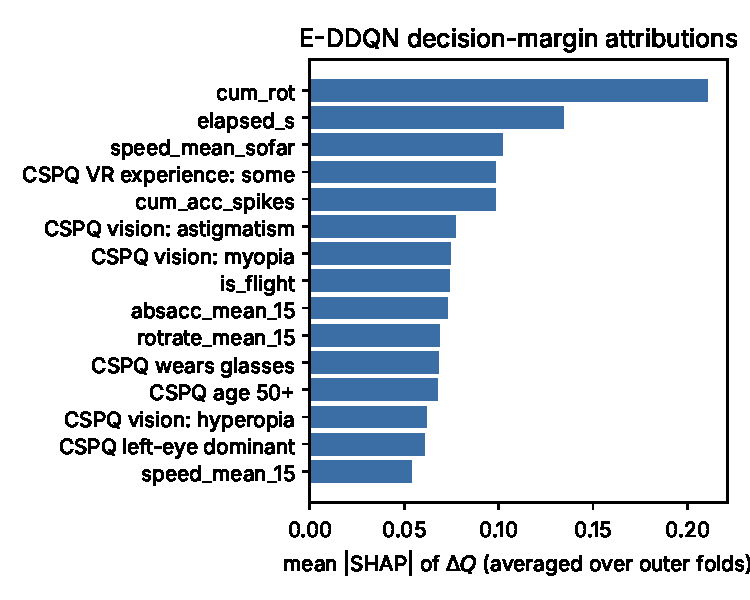
\includegraphics[width=0.6\textwidth]{figs/shap_margin.pdf}
\caption{Mean absolute SHAP value of the E-DDQN decision margin $\Delta Q$ (primary search draw), averaged over the five outer folds.}
\end{figure}

\subsection{Implementation pitfalls of the earlier code}
Three errors are easy to make when a classifier is trained as a Q-learner, and all three were present in an earlier implementation of this study: (i)~transitions built from consecutive rows of shuffled data without terminal flags, so that the next state is an unrelated second, usually of another session; (ii)~the true label stored as the action while the reward of a different, exploratory action is computed (a form of teacher forcing that trains the correct action toward the penalty of the wrong one); (iii)~only the parameters averaged into the target network, so that its batch-normalization statistics never leave their initial values. Unit tests guard against each, and Section~S8 verifies the replay buffer on the real folds.
